\documentclass[a4paper]{article}
\usepackage{amsmath}
\usepackage{bm}
\newcommand\norm[1]{\left\lVert#1\right\rVert}

%% Language and font encodings
\usepackage[english]{babel}
\usepackage[utf8x]{inputenc}
\usepackage[T1]{fontenc}
\usepackage{caption}

%% Sets page size and margins
\usepackage[a4paper,top=3cm,bottom=2cm,left=3cm,right=3cm,marginparwidth=1.75cm]{geometry}

%% Useful packages
\usepackage{amsmath}
\usepackage{graphicx}
\usepackage[colorinlistoftodos]{todonotes}
\usepackage[colorlinks=true, allcolors=blue]{hyperref}

\newcommand{\uvec}[1]{\boldsymbol{\hat{{#1}}}}

\title{Starling Murmurations}
\author{Shubham Singla and Manas Joshi}



\begin{document}
\maketitle

\section{Problem Statement}

Our objective is to design a simulation model for the starling murmurations and compute the average energy spend by each bird, the angular momentum and the force that each bird has to withstand in the phenomenon. We need to computationally simulate the phenomenon by modeling each bird as an independent agent communicating and cooperating with other neighboring agents.
\section{Model}

We have modeled each bird as separate identity which follows some basic rules that results in this amazing phenomenon. Apart from this, the group as a whole needs to make sure that its energy doesn't become infinite and its height is also limited by the ability of the birds to fly as high as possible. 

\subsection{Three basic rules followed by each bird separately }

\medskip
\begin{enumerate}
\item\underline{Cohesion} -  Each bird steer towards average position of neighbours (long range attraction). This means that boids try to fly towards the center of mass of the neighboring boids.
\\\\
\begin{minipage}{\linewidth}
\centering
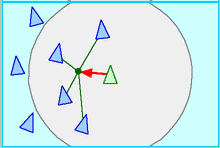
\includegraphics[width=0.3\textwidth]{cohesion.PNG}
\captionof{figure}{Boid moving towards center of mass}
\end{minipage}


\item\underline{Alignment} -  Boids try to match velocity of neighboring boids. A boid steers itself towards the average heading of neighbors.
\\\\
\begin{minipage}{\linewidth}
\centering
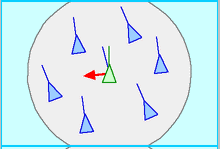
\includegraphics[width=0.3\textwidth]{alignment.PNG}
\captionof{figure}{Boid moving towards average heading of flockmates}
\end{minipage}
\pagebreak
\item\underline{Separation} -  Boids try to keep a small distance away from other objects which includes other boids also. This is done in order to avoid crowding near the neighbors (short range repulsion).
\\\\
\begin{minipage}{\linewidth}
\centering
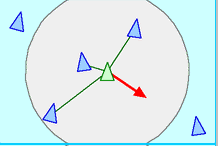
\includegraphics[width=0.3\textwidth]{separation.PNG}
\captionof{figure}{Boid steering away to avoid local crowding}
\end{minipage}

\end{enumerate}



\subsection{Mathematical Analysis}

Consider a bird represented by a point $P_{0}$ in $3D$ space whose position coordinates are given by $(x, y, z)$, velocity at any time $t$ is given by $(v_{x}, v_{y}, v_{z})$ and acceleration is $(a_{x}, a_{y}, a_{z})$. Each bird has some initial energy $E_{o}$ and mass $m_{o}$. We call this entity representing a bird - "boid". When such a boid is flying in the air, it should satisfy the above three rules independently of others. Apart from this, the complete starling needs to follow the basic rules of physics, that is, the energy of the group as a whole can't be more than specified limit which is equal to the sum of the initial energies of each bird in the group.
\\\\
\smallskip
\underline{Mathematical form of the above three rules is stated below - }
\smallskip
\begin{enumerate}
\item\underline{Cohesion} - Let their be a boid - $P_{0}$. It has $N$ neighbours around it. The center of mass of the neighbors is denoted by $CM$ with coordinates are $(x_{cm}, y_{cm}, z_{cm})$. According to the cohesion rule, it tries to move towards $CM$.Let the neighbours be represented by $P_{1}, P_{2}, \ldots, P_{n}$, $CM$ is given by:
	
 
\[CM = \frac{P_1 + P_2 + \cdots + P_n}{n}
      = \frac{1}{n}\sum_{i}^{n} P_i\]
Direction of movement of the bird is given by:
 \[ \uvec{v} = \frac{CM - P_{0}}{\norm {CM - P_{0}}}\]

Let the change in velocity due to cohesion be $\Delta v_{c}$ give by:

\[ \Delta v_{c} = \epsilon \norm{CM - P_{0}} \uvec{v} \]

where, $\epsilon$ is some constant.\\\\

\item\underline{Separation} - Consider a boid represented by point $P_0$. Let its position be $\vec{p_{o}}$ and its neighbours have position $\vec{p_{i}}$. Let $\vec{v}$ be a vector given by:
\[ \vec{v} = \sum_{i}^{} \vec{p_{i}} - \vec{p_{o}}  \qquad \forall\: i, \:\norm{ \vec{p_{i}} - \vec{p_{o}}} < \epsilon' \]

\[ \uvec{v} = \frac{\vec{v}}{\norm{\vec{v}}} \]

where, $\epsilon'$ is some constant. Let the change in velocity due to separation be $\Delta v_{s}$ given by:

\[ \Delta v_{s} = -\epsilon \uvec{v} \]


% \item\underline{Separation} - Consider a bird represented by point $P_0$ is near to k neighbors where near is defined by if the distance between $P_0$ and any other bird is less than some $\epsilon'$. Velocity of the bird is given by $(v_{x}, v_{y}, v_{z})$ and the let the resultant velocity of the birds with which collision is possible is given by $(v'_{x}, v'_{y}, v'_{z})$. Bird should start moving in such a direction that their final velocity is in $-(v'_{x}, v'_{y}, v'_{z})$. Since, it will take $\delta t$ = $\frac{\epsilon'}{\norm{v}}$ amount of time in collision. Acceleration of bird can be found out from the 1st law of motion, that is, 
% \smallskip
% \begin{center}
% $v_{f} = v_{i} + a*(\delta t)$ 
% \end{center}

% where, $a$ denotes the acceleration of the bird. 

\item\underline{Alignment} - The boid steers itself towards the motion of its neighbors. Let the velocity of the neighbors of a boid having velocity $v_{0}$ be defined by $v_{1}, v_{2}, \ldots, v_{n}$. Let the change in velocity due to alignment be $\Delta v_{a}$ given by:
\[ \Delta v_{a} = \epsilon \frac{\sum_{i=1}^{n}(\vec{v_{i} - \vec{v_{0}}})}{\norm{\sum_{i=1}^{n}(\vec{v_{i} - \vec{v_{0}}})}} \]
where, $\epsilon$ is some constant.
% The new velocity of the bird is given by,
% \[v_{f} = \frac{v_1 + v_2 + \cdots + v_n}{n}
%       = \frac{1}{n}\sum_{i}^{n} v_i\]
% Direction of movement of the bird is given by the unit vector - $\frac{v_{f}}{\norm {v_{f}}}$
% \smallskip

% Assuming that the bird moves $\epsilon$ in the above direction given by unit vector.

\end{enumerate}

The new velocity of each boid is given by:
\[ \vec{v_{0}} = \vec{v_{0}} + \Delta \vec{v_{c}} + \Delta \vec{v_{s}}+ \Delta \vec{v_{a}} \]

The new position of each boid is given by:
\[ \vec{x_{0}} = \vec{x_{0}} + \vec{v_{0}}\Delta t  \]

\subsection{Energy Calculation}

\subsubsection{Initial Conditions}

Let each bird have an initial energy $E_{0}$ and mass $m_{0}$.
The simulation starts with $n$ birds each having initial position coordinates  given by :
\[ \boldsymbol{X_{i}} =  \begin{bmatrix} x_{i} & y_{i} & z_{i} \end{bmatrix} ^{T} \]
Let $\mu$ and $\Sigma$ be given by:
\[ \boldsymbol\mu =  \begin{bmatrix} x_{0} & y_{0} & h_{0} \end{bmatrix} ^{T} \]

\[ \boldsymbol\Sigma =  \begin{bmatrix} 
\sigma_{x}^{2} & 0 & 0 \\
0 & \sigma_{y}^{2} & 0 \\
0 & 0 & \sigma_{h}^{2}
 \end{bmatrix} \]
$\boldsymbol{X_{i}}$ comes from a normal distribution:
\[ \boldsymbol{X_{i}} \sim \mathcal{N} (\boldsymbol\mu, \boldsymbol\Sigma) \]
Now we have:

\[ CM_{system_{z}} = \frac{\sum h_{i}}{n} = h_{0}\]
\\
\noindent Similarily, Let the velocity be initialized randomly such that:
\[ v_{system} = \frac{\norm{\sum v_{i}}}{n} = v_{0} \] 
We also have,
\[ \frac{1}{2} m_{0} \sum_{i}^n \norm{v_{i}}^2 + mg \sum_{i}^n h_{i} < nE_{0} \]


\subsubsection{Update Rule}

\noindent At any time $t$, the mechanical energy of boid $i$ is given by:
\[E_{mech, i, t} = \frac{1}{2} m \norm{v_{i, t}}^2 + mgh_{i,t}\] 

\noindent At time $t+1$:
\[E_{mech, i, t+1} = \frac{1}{2} m \norm{v_{i, t+1}}^2 + mgh_{i, t+1}\] 
\\
\noindent Let the energy stored with a boid $i$ at time $t$ be $E_{str, i, t}$, then $E_{str, i, t+1}$ is given by:
\\
\[ E_{str, i, t+1} = E_{str, i, t} - (E_{mech, i, t+1} - E_{mech, i, t}) \qquad (Using\ Energy\ Conservation) \]
\\
\noindent If at any time $t$, $E_{str, i, t} < \epsilon$ for some constant $\epsilon$, then $v_{i,t+1}$ is given by:
\[ v_{i,t+1} = \epsilon' \norm{v_{i,t}}[cosa \uvec{i} + cosb \uvec{j} + cosa \uvec{k}] - v_{z} \uvec{k}, \]
such that,
\[ \norm{v_{i,t+1}} < \norm{v_{i,t}} \] 
$where \ cosa,\ cosb,\ cosc\ are\ direction\ cosines$
%
%
%\subsection{How to add Citations and a References List}
%
%You can upload a \verb|.bib| file containing your BibTeX entries, created with JabRef; or import your \href{https://www.overleaf.com/blog/184}{Mendeley}, CiteULike or Zotero library as a \verb|.bib| file. You can then cite entries from it, like this: \cite{greenwade93}. Just remember to specify a bibliography style, as well as the filename of the \verb|.bib|.
%
%You can find a \href{https://www.overleaf.com/help/97-how-to-include-a-bibliography-using-bibtex}{video tutorial here} to learn more about BibTeX.
%
%We hope you find Overleaf useful, and please let us know if you have any feedback using the help menu above --- or use the contact form at \url{https://www.overleaf.com/contact}!
%
%\bibliographystyle{alpha}
%\bibliography{sample}
%
\end{document}